\documentclass[]{article}
\usepackage{graphicx}

%opening
\title{Bachelorarbeit Zellbewegung}
\author{Fabian Fliedner}

\begin{document}

\maketitle
\begin{abstract}

\end{abstract}

\section{Motivation}
\section{Methoden}
\subsection{Single Cell Tracking}
\subsection{PIV}
\section{Ergebnisse}
\begin{figure}
	\centering
	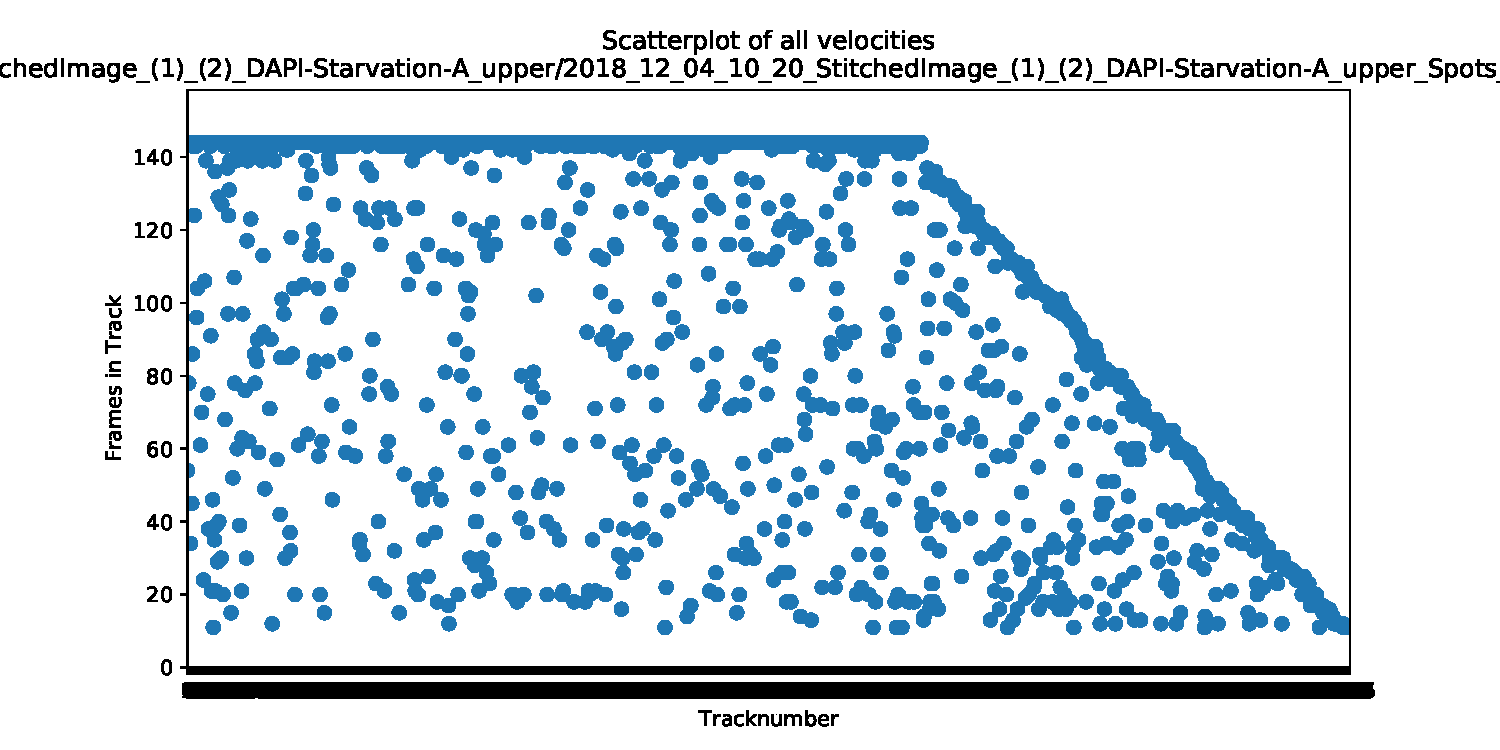
\includegraphics[width=0.7\linewidth]{BildDateien/length_of_all_tracks}
	\caption[Tracklänge nach ID]{Länge der Tracks in von der ID}
	\label{fig:lengthofalltracks}
\end{figure}


\end{document}
